\section{Use-Cases}
\subsection{Frontend}
\begin{figure}[ht]
  \centering
  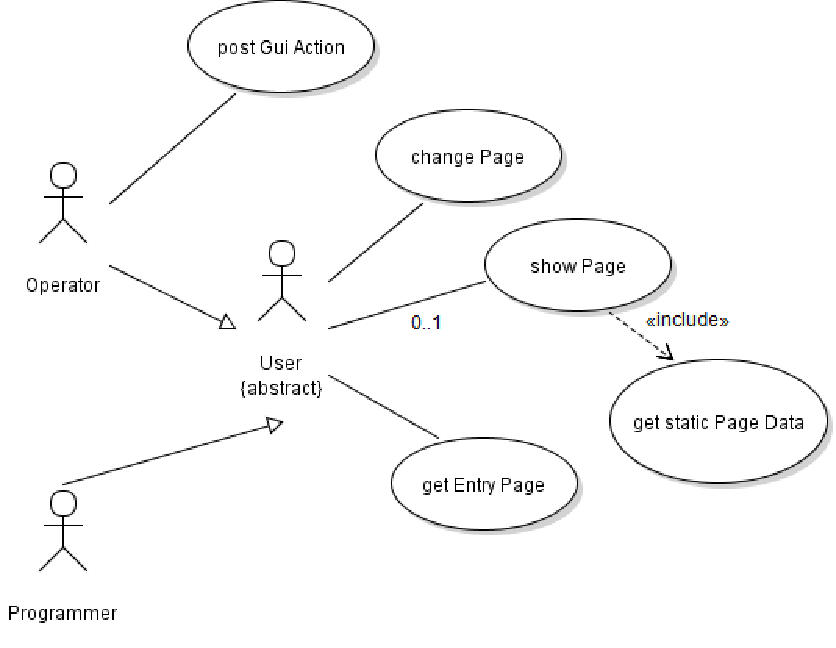
\includegraphics[width=0.9\textwidth]{content/hauptteil/systemEntwurf/res/frontendUseCase.pdf}
  \caption[Use-Case Diagramm des Frontends]{Use-Case Diagramm des Frontends}
  \label{img:beUC}
\end{figure}
Aus der Zielsetzung der Arbeit ergibt sich das Use-Case Diagramm in Abbildung \ref{img:feUC}.
Das Diagramm beschreibt abstrakt die Anwendungsfälle die das \ac{scada} System für den Anwender in der Rolle des Bedieners (Operator), 
sowie des Programmierers (Programmer) erfüllen muss.

\subsection{Backend}
\begin{figure}[ht]
  \centering
  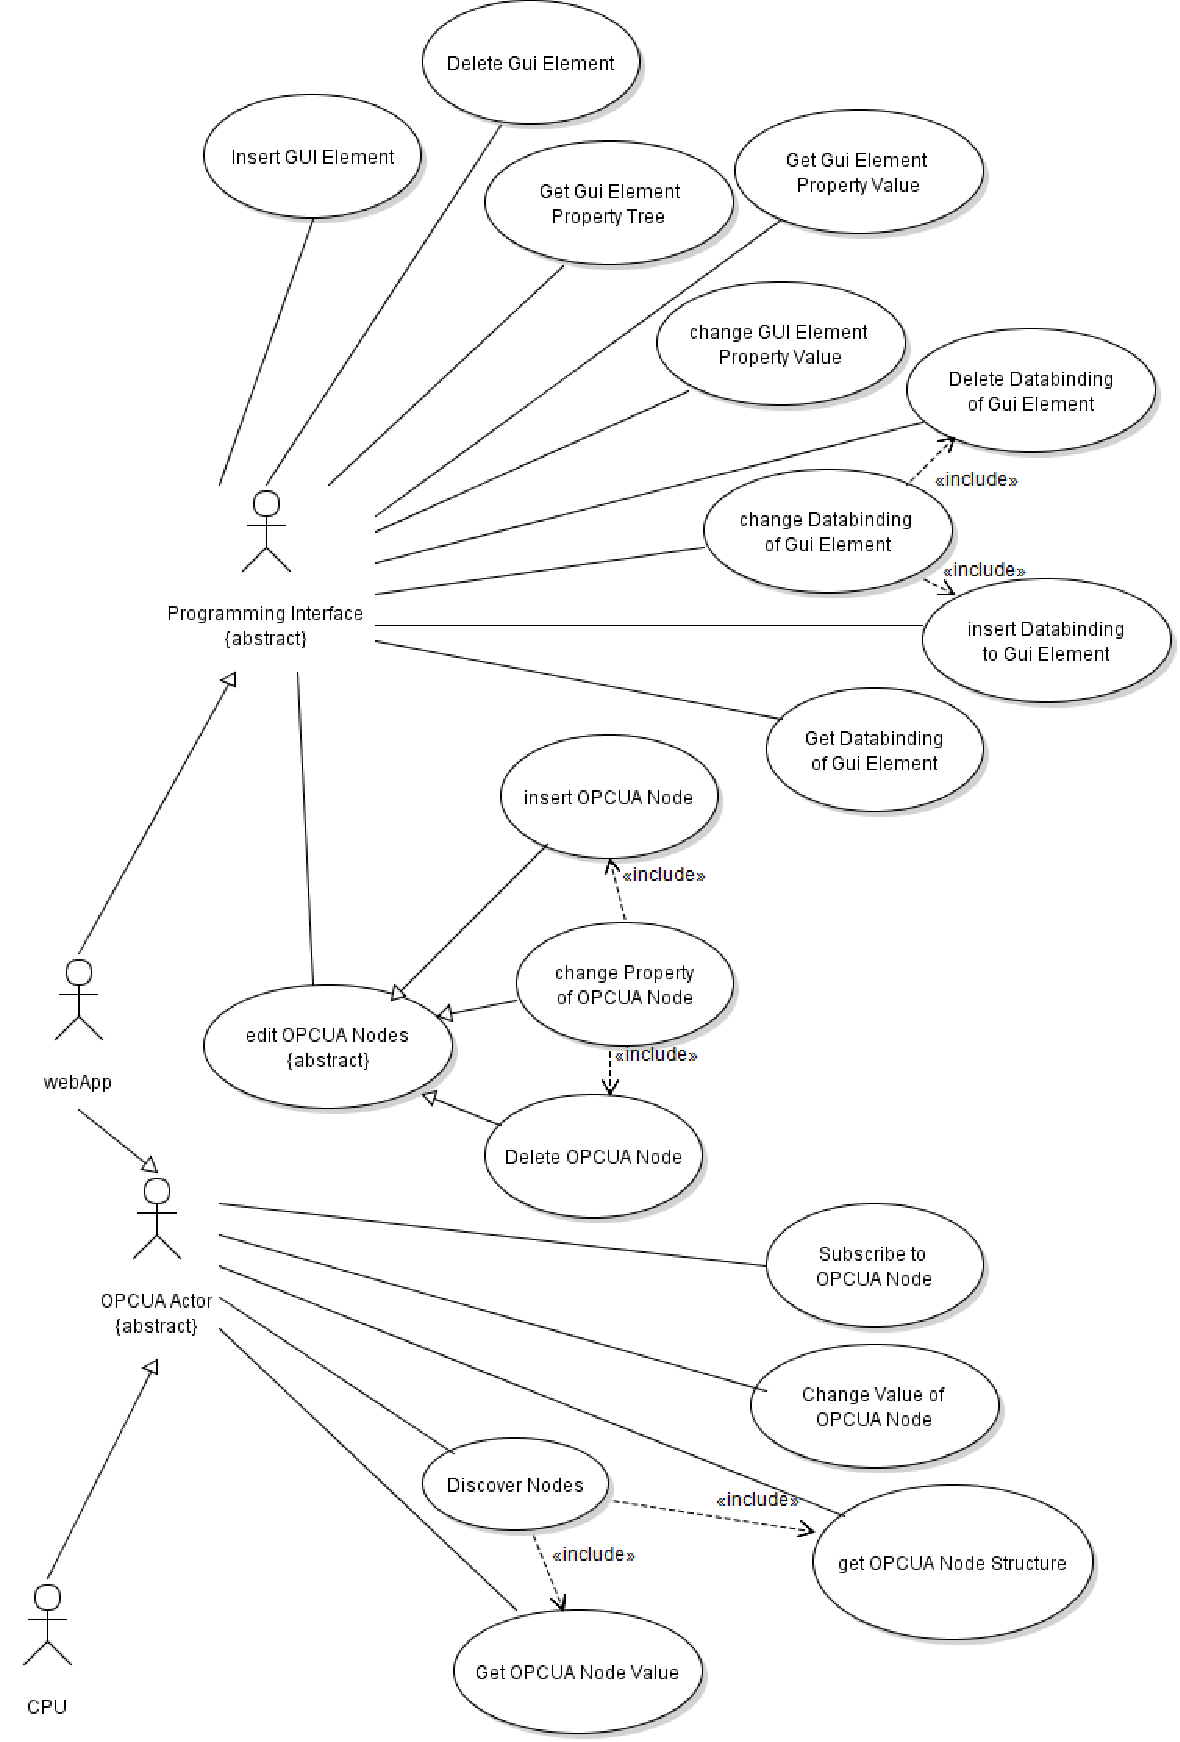
\includegraphics[width=\textwidth]{content/hauptteil/systemEntwurf/res/backendUseCase.pdf}
  \caption[Use-Case Diagramm des Backends]{}
  \label{img:feUC}
\end{figure}
Aus der Zielsetzung der Arbeit ergibt sich das Use-Case Diagramm für das Backend in Abbildung \ref{img:feUC}.